\documentclass[a4paper, 11pt]{report}
\usepackage{blindtext}
\usepackage[T1]{fontenc}
\usepackage[utf8]{inputenc}
\usepackage{titlesec}
\usepackage{fancyhdr}
\usepackage{geometry}
\usepackage{fix-cm}
\usepackage[hidelinks]{hyperref}
\usepackage{graphicx}
\usepackage{titlesec}
\usepackage{cite}
\usepackage[english]{babel}

\geometry{ margin=30mm }
\counterwithin{subsection}{section}
\renewcommand\thesection{\arabic{section}.}
\renewcommand\thesubsection{\thesection\arabic{subsection}.}
\usepackage{tocloft}
\renewcommand{\cftchapleader}{\cftdotfill{\cftdotsep}}
\renewcommand{\cftsecleader}{\cftdotfill{\cftdotsep}}
\setlength{\cftsecindent}{2.2em}
\setlength{\cftsubsecindent}{4.2em}
\setlength{\cftsecnumwidth}{2em}
\setlength{\cftsubsecnumwidth}{2.5em}

\titlespacing\section{0pt}{12pt plus 4pt minus 2pt}{0pt plus 2pt minus 2pt}
\titlespacing\subsection{0pt}{12pt plus 4pt minus 2pt}{0pt plus 2pt minus 2pt}

\begin{document}
\titleformat{\section}
{\normalfont\fontsize{15}{0}\bfseries}{\thesection}{1em}{}
\titlespacing{\section}{0cm}{0.5cm}{0.15cm}
\titleformat{\subsection}
{\normalfont\fontsize{13}{0}\bfseries}{\thesubsection}{0.5em}{}
\titlespacing{\section}{0cm}{0.5cm}{0.15cm}

%=============================================================================

\pagenumbering{Alpha}
\begin{titlepage}
\begin{flushright}

\includegraphics[width=4cm]{USyd}\\[2cm]
\end{flushright}
\center 
\textbf{\huge INFO1111: Computing 1A Professionalism}\\[0.75cm]
\textbf{\huge 2023 Semester 1}\\[2cm]
\textbf{\huge Self-Learning Report}\\[3cm]

\textbf{\huge Submission number: 3}\\[0.75cm]
\textbf{Github link: \url{https://github.sydney.edu.au/INFO1111-2023/Self-learning-for-Yizhen-Pan}}\\[2cm]

{\large
\begin{tabular}{|p{0.35\textwidth}|p{0.55\textwidth}|}
	\hline
	{\bf Student name} & Yizhen Pan\\
	{\bf Student ID} & 520009998\\
	{\bf Topic} & JavaScript \\
	{\bf Levels already achieved} & A\\
	{\bf Levels in this report} & B,C\\
	\hline
\end{tabular}
}
\thispagestyle{empty}

\pagenumbering{arabic}
\end{titlepage}

%=============================================================================

\newpage
\section{Level A: Initial Understanding}
\vspace{5mm}
\subsection{Level A Demonstration}

1. Install WebStorm IDE and create a JavaScript project

2. the project will include a JavaScript function and a web page to embed the function 

3. one text box, which collect the message, will be provided in the web page for JavaScript function to do.

4. three trigger based (button will be working as it is clicked) buttons will be created, one button will store 
the information for function to use and other two buttons will use different functions as it clicked.

\subsection{Learning Approach}

First, I install the WebStorm IDE, a good tool for me to work and demonstrate JavaScript. 
Then I started to look over the contents about JavaScript by googling some online courses about JavaScript,  
the website I use to help 
archive the study is w3school, \cite{w3school} gives me a clear instructions on how to study and use JavaScript 
from the start, furthermore, \cite{w3school} also provides a simple JavaScript simulator which helps me to use 
the knowledge I learned directly. 
\\

After learning basic knowledge to set up a JavaScript function, I googled the content about the use of different 
<Input> in HTML and the way to combine it with JavaScript. The website I used for this part is mdn web docs, a 
website teaching the contents of HTML. \cite{input} shows different attributes of input, greatly help me 
understanding the use of <input>. 
\\

After all the studies, I used WebStorm IDE to create a JavaScript Project, which contains a js file and an HTML 
file, and demonstrate the Level A demonstration steps I implement above to show my understanding of JavaScript.


\subsection{Challenges and Difficulties}

I think the challenge parts are receiving inputs, setting the variables and the way to use them into the function. 

The ways for JavaScript to receive messages from users and output results are quite different from Python or Java 
that I learned. As \cite{input} and \cite{w3school} mentioned, we can use <input> with different attributes to 
get the correct type of message that we want in the HTML; like for the rotation part, I set the attribute to only 
receive integer numbers from 1 to 25. However, the message part is quite different since users may implement 
messages that combine Upper and Lower cases or even other signatures, increasing the difficulty to rotate them 
correctly. I solve the difficulty by converting them to ASCII code to rotate and then converting them back to 
text. This way greatly helped solve the problem a lot, but I also got into another problem, which was the 
position to rotate. This caused me to get the wrong rotation message. finally, I set the position to the mid-
point of the alphabet letters to shift.

\subsection{Learning Sources}

\begin{tabular}{|p{0.45\textwidth}|p{0.45\textwidth}|}
	\hline
	Learning Source  & Contribution to Learning\\
	\hline
	\url{https://www.w3school.com.cn/js/index.asp} & this website introduced me the basic knowledge of JavaScript\\
	\hline
	\url{https://developer.mozilla.org/en-US/docs/Web/HTML/Element/input} & it give me some ideas of how to use different ways of getting input from users\\
	\hline
	\url{https://en.wikipedia.org/wiki/Caesar_cipher} & it describes the function I want to demonstrate and the idea of how it works\\
	\hline
\end{tabular}

\subsection{Application artifacts}
The application I created is a web page that does Caesar cipher encryption.

The idea of Caesar cipher described by \cite{caesar} is a type of substitution cipher in which each letter in the plain text is replaced by a letter some fixed number of positions down the alphabet.

The way it works in my application is by entering the message, which need to encrypt, and then enter the number to rotate, and then click encrypt button to receive the processed encrypt message.

The function encrypt takes input from two HTML input elements with IDs $message$ and $rot$, respectively. The input message is stored in the variable $str$, and the rotation amount is stored in the variable $rt$, then creates an empty string, $new_str$, which will store the encrypted message. The function loops through each character in the input $str$ using a for loop.

For each character, the function checks whether it is a letter or not using the $charCodeAt()$ method. If the 
character is an uppercase letter (ASCII code between 65 and 90) or a lowercase letter (ASCII code between 97 and 
122), it is rotated by the value of rt using a simple Caesar cipher, where each letter is shifted rt positions to 
the right. 
The modulo operator $\%$ is used to wrap around the alphabet so that letters beyond Z or z wrap back to A or a. All the rotated letters are added to $new_str$.

If the character is not a letter, the function simply adds the character to $new_str$ without rotation.

Finally, the encrypted message is output to an HTML element with ID $result$ using the innerHTML method.

Coding part is showed in the graph below:

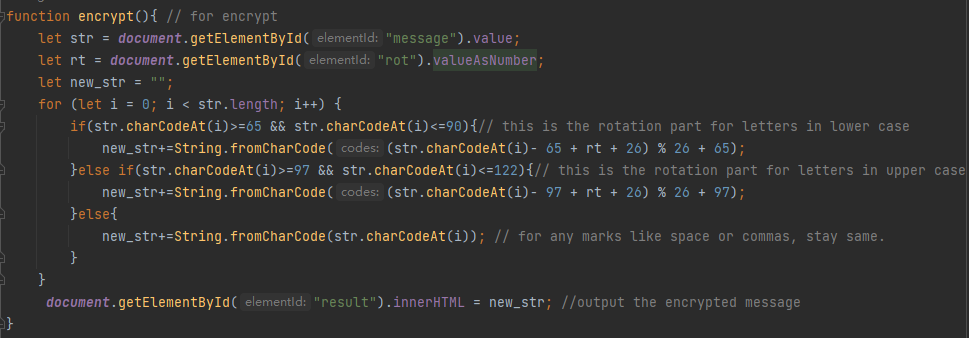
\includegraphics[width=14cm]{screengrabs/JavaScript encrypt.png}

%=============================================================================

\newpage
\section{Level B: Basic Application}

\subsection{Level B Demonstration}
The application I develop is a simple Caesar Cipher web page that can do both message encryption and decryption, the web page contains two event based triggers, encrypt and decrypt, that works as the button clicked by the user, two input text boxes--one for enter message, one for enter rotation value.

\subsection{Application artifacts}

In HTML part, JavaScript functions are activated when user click the button decrypt or encrypt, and the encrypt()
and decrypt() functions in the JavaScript get the message and rot value entered by the user after the click using 
document.getElementById("message").value and document.getElementById("rot").valueAsNumber. The result will be 
showed after the line of button.

Example output

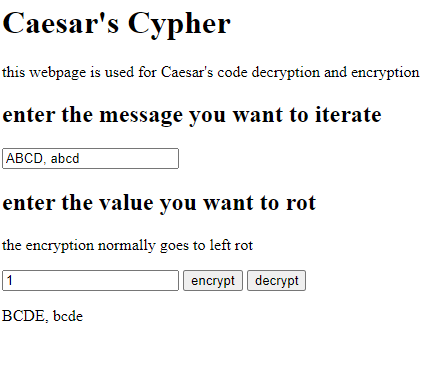
\includegraphics{screengrabs/result for encryption.png}

the complete HTML codes are showed below

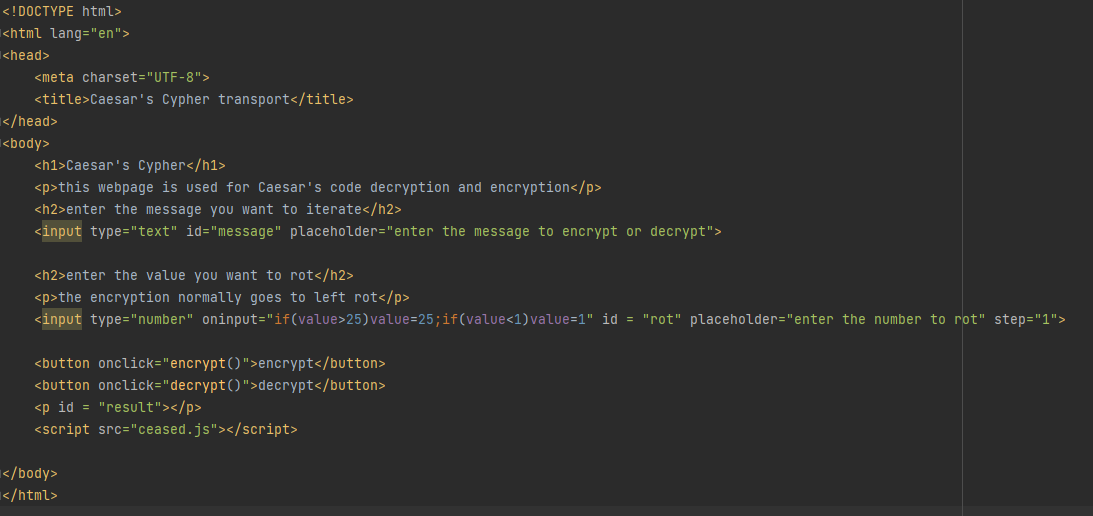
\includegraphics[width=14cm]{screengrabs/HTML code.png}

the complete JavaScript codes are showed below

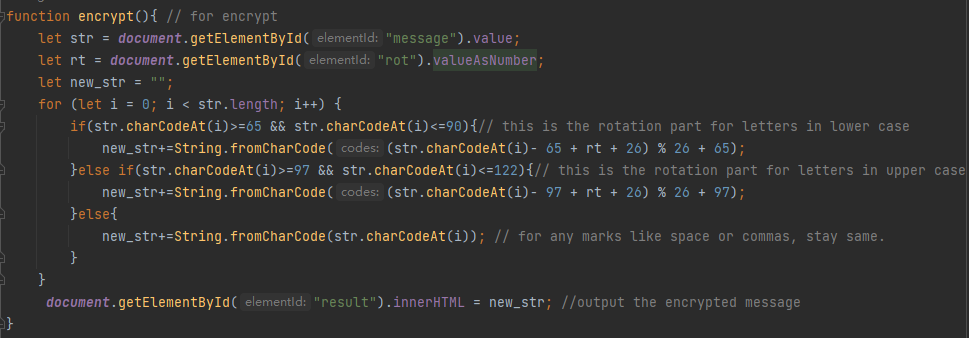
\includegraphics[width=14cm]{screengrabs/JavaScript encrypt.png}

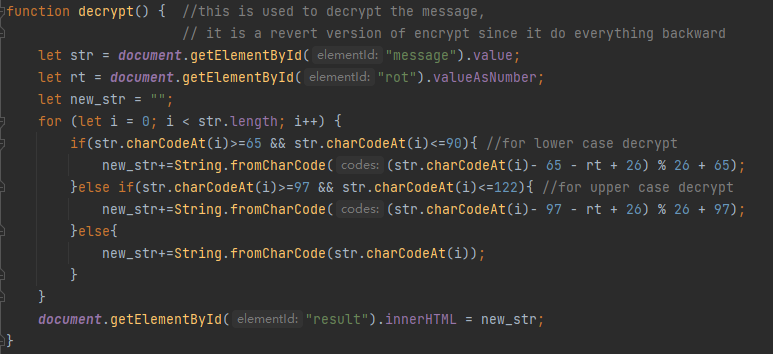
\includegraphics[width=14cm]{screengrabs/JavaScript decrypt.png}

%=============================================================================

\newpage
\section{Level C: Deeper Understanding}

%Level C focuses on showing that you have actually understood the tool or technology at a relatively advanced level. You will need to compare it to alternatives, identifying key strengths and weaknesses, and the areas where this tool is most effective. 

\subsection{Strengths}
%What are the key strengths of the item you have learnt? (50-100 words)
According to \cite{geeksforgeeks-2023B} and my personal experience from developing the project, the key strengths are listed below:

1. JavaScript is very fast since it executes on the client side and this also reduces the server load since it can produce an error message before any information is transmitted to the server.

2. JavaScript is used everywhere on the web and can be execute in any modern browsers and produce equivalent results.

3. JavaScript plays nicely with other languages and utilized in an enormous sort of applications. 

4. There are a lot of open-source projects and online courses about JavaScript, making it become one of the easiest IT languages to learn.

\subsection{Weaknesses}
%What are the key weaknesses of the item you have learnt? (50-100 words)
The weaknesses of JavaScript is also very obvious too according to \cite{geeksforgeeks-2023B}  

1. JavaScript codes are always visible to the client side, as we can simply use F12 in the browser to look at the source code. This can open up avenues of attack for malicious parties looking to gain access to related systems, do damage, or deny others access.

2. Compared to other programming languages, JavaScript is less strict on conventions and rules. For example, Java has String, int, float, char, and Boolean types to initialize the variables, but JavaScript may only use var to initialize all the types of variables needed to use, which may lead developers to bad habits if they aren't careful about applying rules of their own.

3. the websites powered by JavaScript can be displayed differently in different browsers. This makes it somewhat complex to read and write cross-browser code.

\subsection{Usefulness}
%Describe one scenario under which you believe the topic you have learnt could be useful. (50-100 words)
One such scenario I think JavaScript could be useful is in web development. According to \cite{pedamkar-2023}'s description, JavaScript is used when a webpage is to be made dynamic and add special effects on pages like rollover, roll out and many types of graphics since JavaScript will be executed immediately when user enter the web page.

\subsection{Key Question 1}
%Note: This question is in the table in the ‘Self Learning: List of Topics’ page on Canvas. (50-100 words)
% When should you use javascript? Not use javascript?
when to use it:

Based on \cite{coyier-2009} and \cite{pedamkar-2023} descriptions, one of the right time to use JavaScript is in web development, especially the user need to have their website communicate with the browser and watch for events like clicks and mouse enters since JavaScript is available for having the website interact with the browsers and users immediately.

not to use it:

JavaScript is not appropriate to use in creating Security-Sensitive Applications since one of the weaknesses of JavaScript is the codes are always visible to the client side, which will cause significant cybersecurity issues since we don't want users to access the sensitive information that might be included in the codes.


\subsection{Key Question 2}
%Note: This question is in the table in the ‘Self Learning: List of Topics’ page on Canvas. (50-100 words)
% How does javascript make use of frameworks?
According to \cite{brewster-no-date} and \cite{codemotion-2023}'s descriptions, JavaScript Frameworks are collections of different JavaScript code libraries that are compiled together to make it easy for a developer to refer to and use the scripts; It can greatly help developers to create websites easier. In the meantime, developers can choose the proper JavaScript frameworks to suit their needs, whether is the right size and performance, the one most compatible in the backend, or the right level of complexity.

%=============================================================================

\newpage
\section{Level D: Evolution of skills}
\vspace{5mm}
\subsection{Level D Demonstration}

% This is a short description of the application that you have developed. (50-100 words).
% \textit{{\bf IMPORTANT:} You might wish to submit this as part of an earlier submission in order to obtain feedback as to whether this is likely to be acceptable for level D.}

\subsection{Application artifacts}

% Include here a description of what you actually created (what does it do? How does it work? How did you create it?). Include any code or other related artefacts that you created (these should also be included in your github repository).

% If you do include screengrabs to show what you have done then these should be annotated to explain what it is showing and what the application does.

\subsection{Alternative tools/technologies}
% Identify 2 alternative tools/technologies that can be used instead of the one you studied for your topic. (e.g. if your topic was Python, then you might identify Java and Golang)
\subsection{Comparative Analysis}
% Describe situations in which both your topic and each of the identified alternatives would be preferred over the others (100-200 words).



%=============================================================================

\newpage
 
\bibliographystyle{IEEEtran}
\bibliography{main}

\end{document}
\end{report}
